% N-state model chapter.
%%%%%%%%%%%%%%%%%%%%%%%%

\chapter{The N-state model or ensemble analysis} \label{ch: N-state model}
\index{N-state model|textbf}
\index{Ensemble analysis|textbf}


\begin{figure*}[h]
  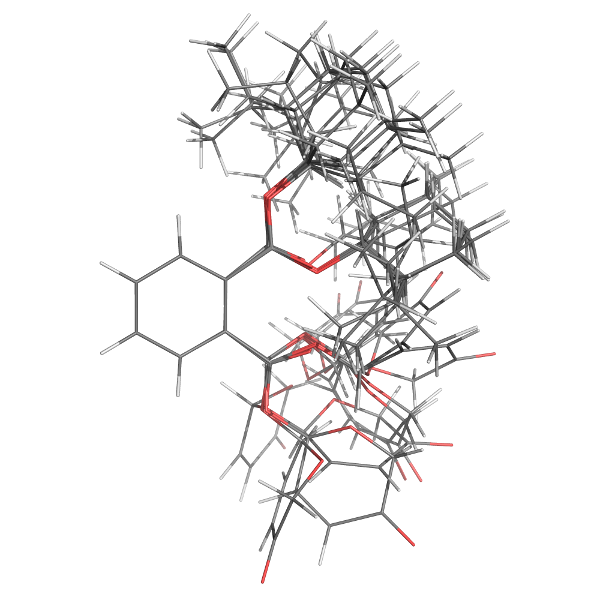
\includegraphics[width=5cm, bb=0 0 1701 1701]{graphics/misc/n_state_model/phthalic_acid_ens_600x600}
\end{figure*}


% Introduction.
%%%%%%%%%%%%%%%

\section{Introduction to the N-state model}

The modelling of motion in molecules using experimental data consists of either continuous or discrete distributions.
These can be visualised respectively as either an infinite number of states or a limited set of N states.
The N-state model analysis in relax models the molecular dynamics using an ensemble of static structures.

This analysis supports a number of data types including:
\begin{itemize}
\item Residual dipolar couplings (RDCs)\index{Residual dipolar coupling}
\item Pseudo-contact shifts (PCSs)\index{Pseudo-contact shifts}
\item NOEs\index{NOE}
\end{itemize}

The main idea is to evaluate the quality of a fixed ensemble of structures.
relax will not perform structural optimisations.
The evaluation includes:
\begin{itemize}
\item Alignment tensor optimisation for the RDCs and PCSs.
\item Optional optimisation of the position of the paramagnetic centre for the PCSs.
\item Calculation of NOE constraint violations.
\item Q factor calculation for the RDC, PCS, and NOE.
\end{itemize}

Note that this analysis will also handle single structures.
Hence you can use the N-state model in relax with N set to 1 to find, for example, a single alignment tensor for a single structure using RDCs, PCSs, or both together.
This is useful for comparing a ensemble to a single structure to determine if any statistically significant motions are present.

The primary references for the N-state model analysis in relax are:
\begin{itemize}
  \item \bibentry{Sun11}
  \item \bibentry{Erdelyi11}
\end{itemize}



% Data types.
%%%%%%%%%%%%%
 
\section{Experimental data support for the N-state model}

% RDCs.
\subsection{RDCs in the N-state model}

Residual dipolar couplings (RDCs)\index{Residual dipolar coupling|textbf} can be used to evaluate ensembles.  
The ensemble interconversion is assumed to be fast relative to timescale of the alignment process, hence a single tensor for all members of the ensemble will be used.
As such, precise superimposition of structures using a logical frame of reference is very important.
This can be performed in relax using the \uf{structure\ufsep{}superimpose} user function.
The RDCs can either be from external or internal alignment.


% PCSs.
\subsection{PCSs in the N-state model}

Pseudo-contact shifts (PCSs)\index{Pseudo-contact shifts|textbf} can also be used to evaluate ensembles.  
The same averaging process as described above for the RDC is assumed.
Hence correct structural superimposition is essential and one alignment tensor will be optimised for the entire ensemble.

One powerful feature of relax is that the paramagnetic centre can either be fixed or be allowed to move during optimisation.
This allows an unknown paramagnetic centre position to be found.
Or a known position to be refined to higher accuracy than that possible with most other techniques.


% NOEs.
\subsection{NOEs in the N-state model}

Another data type which can be used to evaluate dynamics ensembles is the NOE\index{NOE|textbf}.
This is not used in optimisation but rather is used to calculate NOE constraint violations.
These violations are then compared to evaluate the ensemble.
In the stereochemistry auto-analysis, these violations will also be converted to Q factors to allow direct comparison with RDC Q factors.
